% \documentclass[12pt, twoside]{article}
\usepackage[letterpaper, margin=1in, headsep=0.2in]{geometry}
\setlength{\headheight}{0.6in}
%\usepackage[english]{babel}
\usepackage[utf8]{inputenc}
\usepackage{microtype}
\usepackage{amsmath}
\usepackage{amssymb}
%\usepackage{amsfonts}
\usepackage[nomessages]{fp} %\FPeval{\var-name}{2*sin(pi/6)}
\usepackage{siunitx} %units in math. eg 20\milli\meter
\usepackage{yhmath} % for arcs, overparenth command
\usepackage{tikz} %graphics
\usetikzlibrary{quotes, angles, arrows, arrows.meta}
\usepackage{graphicx} %consider setting \graphicspath{{images/}}
\usepackage{parskip} %no paragraph indent
\usepackage{enumitem}
\usepackage{multicol}
\usepackage{venndiagram}

\usepackage{fancyhdr}
\pagestyle{fancy}
\fancyhf{}
\renewcommand{\headrulewidth}{0pt} % disable the underline of the header
\raggedbottom
\hfuzz=2mm %suppresses overfull box warnings

\usepackage{hyperref}

\fancyhead[LE]{\thepage}
\fancyhead[RO]{\thepage \\ Name: \hspace{4cm} \,\\}
\fancyhead[LO]{BECA / Dr. Huson / Geometry\\*  Unit 6: Analytic geometry\\* 23 November 2022}

\begin{document}

\subsubsection*{6.3 Classwork: Standard form of a linear equation}
Equations of a straight line: $f(x)=mx+c$, $ax+by+d=0$, $(y-y_1)=m(x-x_1)$\\[0.25cm]
Gradient: $\displaystyle m=\frac{y_2-y_1}{x_2-x_1}$ \vspace{1cm}
\begin{enumerate}
\item A linear equation $f$ is graphed below.
\begin{multicols}{2}
\begin{enumerate}
  \item Write down it's slope.\\ $m=$
  \vspace{0.25cm}
  \item Write down it's $y$-intercept.\\ $b=$
  \vspace{0.25cm}
  \item Write down the equation of the line.
  \vspace{1cm}
  \item State the coordinates of the point $P$.
\end{enumerate} \vspace{.5cm}
  \begin{center} 
  \begin{tikzpicture}[scale=0.8]
    \draw [help lines] (-3,-2) grid (4,6);
    \draw [thick, ->] (-3.2,0) -- (4.4,0) node [below right] {$x$};
    \draw [thick, ->] (0,-2.2)--(0,6.4) node [left] {$y$};
    \foreach \x in {-3,-2,-1,1,2,...,4} \draw (\x cm,1pt) -- (\x cm,-1pt) node[anchor=north] {$\x$};
    \foreach \y in {1, 2, 3, 4, 5} \draw (1pt,\y cm) -- (-1pt,\y cm) node[anchor=east] {$\y$};
    \draw [thick, <->] (-0.25,-1.5) -- (3.25,5.5);
    \fill (2,3) circle[radius=0.1] node[below right]{$P$};
  \end{tikzpicture}
  \end{center}
\end{multicols}

\item Write the linear equation $y-2=3(x+1)$ in the form $y=mx+c$. \vspace{4cm}

\item A line has a gradient (slope) of $\displaystyle -\frac{3}{2}$ and passes through the point $(4, 1)$. Find the equation of the line in the form $y=mx+b$.

\newpage
\item A line goes through the points $(2, 3)$ and $(5, 12)$.
\begin{enumerate}
  \begin{multicols}{2}
      \item Find the gradient of the line.
      \item Find the equation of the line in the form $y=mx+b$.\vspace{2cm}
      \begin{center}
      \begin{tikzpicture}[xscale=0.7, yscale=0.4]
        %\draw [help lines] (-3,-2) grid (4,6);
        \draw [thick, ->] (-1.2,0) -- (7.4,0) node [below right] {$x$};
        \draw [thick, ->] (0,-1.2)--(0,13.5) node [right] {$y$};
        \foreach \x in {-1, 1,2, ..., 7} \draw (\x cm,4pt) -- (\x cm,-4pt) node[anchor=north] {$\x$};
        \foreach \y in {2, 4, ..., 12} \draw (2pt,\y cm) -- (-2pt,\y cm) node[anchor=east] {$\y$};
        \fill (2,3) circle[radius=0.1] node[below right]{$(2,3)$};
        \fill (5,12) circle[radius=0.1] node[below right]{$(5,12)$};
        \draw [thick, <->] (1.67,2)--(5.33,13);
      \end{tikzpicture}
      \end{center}
    \end{multicols}
\end{enumerate} \vspace{3cm}

\item Find the equation of the line through the points $(4, 3)$ and $(-2, 18)$. 


\end{enumerate}
\end{document}